\chapter{Theoretical framework}
\label{cha:chapter 2}

On this section we present concepts to support and further explain the technologies and process found on the Methodology and Development section. We present concepts regarding spatial networks and its analysis measures based on network theory; spatial data; as well as some tools and services that we use as a base for this work.

\section{Spatial Networks}
A network (or \textit{graph} in mathematics) is composed of nodes $N$ connected by links, or edges, $E$. Nodes represent entities in a network, such as cities, people, airports, and street intersections. Edges represent relationship between nodes, such as friendships among people, flights between airports, street roads, and so on. 

Graphs can be arranged nonspatially or spatially. Spatial graphs have nodes that are georeferenced, i.e. they are defined by their location in geographic space using a pair of coordinates; usually embedded in a two- or three-dimensional space \cite{barthelemy_spatial_2011}. Both nonspatial and spatial graphs can contain undirected, directed, unweighted, or weighted components \cite{anderson_2020}.

An undirected graph has edges that can be used to represent flows of traffic on two-way streets, while edges in a directed graph represent one-way streets. A self-loop in a graph is an edge that connects a single node to itself. Two nodes can also be connected by parallel edges, in such case, graphs are called multigraphs, or multidigraphs if they are directed. The weight attribute in a weighted graph is used to quantify some value between connected nodes \cite{boeing_osmnx_2017}.

Network science was founded on the based on the findings by Euler \cite{euler_1741}, and gave way to the notion that graphs have different structural properties that can be discovered and cataloged using graph theory \cite{barabasi_2016}. With this, early spatial network analysis focused on using graph theory and its measures to describe and catalog the properties of real systems represented as spatial networks \cite{anderson_2020}. 

Real spatial networks are complicated physical entities, with numerous, often complex, elements with a nontrivial configuration and structure that are neither purely fully regular nor fully random. A street network is an example of a complex spatial network with both nodes and edges embedded in space.

A spatial network is \textit{planar} if it can be represented in two dimensions with its edges intersecting only nodes. A street network may be planar at certain small scales, but most street networks are non-planar due to overpasses, bridges, tunnels, etc. For tractability, these networks are studied as approximately planar. However, it can cause analytical problems due to the over-simplification.

Street networks can be based on two graph representations: primal graph or dual graph. In a primal graph representation, intersections are turned into nodes and street segments into edges. On the other hand, dual graphs invert the representation: streets as nodes and intersections as edges \cite{porta_streets_2006}. Primal graphs retain all the geographic, spatial information that are lost in a dual graph. For that reason, primal representation is the better approach for analyzing spatial networks as it faithfully represents all the spatial characteristics of a street \cite{ratti_spacesyntax_2004}.

\section{Spatial Networks Analysis Measures}

The structure and behavior of networks can be described using a variety of graph theory measures. These measures can be found in different level of detail in \cite{barabasi_2016, barthelemy_spatial_2011, lewis_2011, newman_2004, newman_2010, menczer_fortunato_davis_2020}.

Each network is characterized by the \textbf{total number of nodes} $N$ and the \textbf{total number of edges} $E$. We call $N$ the \textbf{size of the network}. 

The \textbf{\textit{degree}} $k$ of a node is its number of edges, or neighbors, and it is a local measure. We use $k_i$ to denote the degree of node $i$. A node with no neighbors has degree zero ($k = 0$) and is called a \textbf{\textit{singleton}}.

The \textbf{average degree} $<k>$ is a global measure for the average degree $k$ across all nodes $N$ in a graph. This measure is simplified by dividing twice the number of edges $E$ by the number of nodes $N$, as follows:

\begin{equation} \label{eq:1}
<k> = \frac{2E}{N}
\end{equation}

The average streets per node measures the mean number of streets (edges in an undirected graph) that come out from each intersection or dead-end.

The \textbf{degree distribution} $P(k)$ represents the fraction of nodes in a graph with degree $k$, calculated by dividing the number of nodes with degree $k$ by the total number of nodes $N$ in the graph $G$. The degree distribution $P(k)$ is often plotted on a histogram and is useful for providing an overall snapshot of graph $G$.

The \textbf{clustering coefficient} $C$ measures the ability of an individual node $i$ to associate with other nodes (cliquishness). It is commonly described as the probability that "friends" of $i$ (i.e., nodes connected to node $i$) are also friends of each other: the chance that a friend of my friend is also my friend \cite{watts_strogatz_1998}. For node $i$ of degree $k_i$, the clustering coefficient $C(i)$ is defined as:

\begin{equation} \label{eq:2}
	C(i) = \frac{E_i}{k_i(k_i - 1)/2}
\end{equation}

where $E_i$ is the number of edges existing between the neighbors of $i$. When the local measure $C = 1$, the node $v_i$ and its neighboring nodes are all perfectly connected. In contrast, when $C = 0$, neighbors of node $i$ are not connected at all.

The \textbf{average clustering coefficient} $<C>$ is a global measure that determines the cliquishness of all nodes in a graph and is calculated as the average $C$ over all individual nodes. When $<C> = 1$, the graph is perfectly connected. In contrast, when $<C> = 0$, the graph is not connected at all.

\textbf{Path} $P$ is and ordered sequence, or collection, of edges that connects some ordered sequence of nodes. The collection of nodes $N$ and edges $E$ in a path can be defined as:

\begin{equation} \label{eq:3}
N_p = \{0,1,2,...n\}
\end{equation}

\begin{equation} \label{eq:4}
E_p = \{0,1,2,...m\}
\end{equation}

There may be many paths of varying lengths $l$ between two nodes $i$ and $j$. The \textbf{shortest path length} $l_s$ is calculated by counting the total number of intermediate nodes or edges along the shortest path between two nodes $i$ and $j$ and is defined as:

\begin{equation} \label{eq:5}
	l_s(i,j) = \min_\text{paths}({i \to j})
\end{equation}

The \textbf{average shortest path length} $<l>$ is defined as the average shortest path length between all possible pairs of nodes in the network. The \textbf{diameter} $d_G$ of a graph $G$ is defined as the maximum shortest path length $l_s$ found in the graph.

\textbf{Average street length} is the mean edge length measured in meters, an example of spatial units, and indicates how fine-grained (small block size) or coarse-grained (large block size) the networks is.

Density measures provided how fine-grained the network is. \textbf{Node density} is the number of nodes divided by the area covered by the network. \textbf{Intersection density} is the node density of the set of nodes with more than one street emanating from them, excluding dead-ends. The \textbf{edge density} is the sum of all edge lengths divided by the area. The physical \textbf{street density} is the sum of all edges (in the undirected graph) divided by the area.

The \textbf{average circuity} is the circle distances between the nodes of each edge, and it is defined by the sum of all edge lengths divided by the sum of the great-circle distances between the nodes incident to each edge \cite{giacomin-levinson_2015}.

\textbf{Eccentricity} is the largest distance (the maximum of the shortest-path weighted distances) between a node and other nodes i.e., how far the node is from the node that is furthest from it \cite{urban-keitt_2001}. The \textbf{diameter} of a network is the maximum eccentricity of any node in the network and the \textbf{radius} is the minimum eccentricity \cite{hage-harary_1995}. The \textbf{center} if a network is the node or set of nodes with an eccentricity equals the radius, and the \textbf{periphery} of a network is the node or set of nodes with eccentricity equals the diameter. These distances serve as indicators for network size and shape if we use length as weight. 

\textbf{Connectivity} measures the minimum number of nodes or edges that must be removed from a connected graph to disconnect the network \cite{urban-keitt_2001}. In the case of street networks, we use \textbf{average node connectivity} as a resilience indicator, which is the mean number of internally node-disjoint paths between each pair of nodes. This measure is more useful to represent the expected number of nodes that must removed to disconnect a randomly selected pair of non-adjacent nodes \cite{beineke-oellermann-pippert_2002, dankelmann-oellermann_2003} Networks with low connectivity may have multiple points of failure, this yield to a vulnerable system. 

Centrality measures indicate the most important nodes in a network \cite{huang_2016, zhong_2017}. \textbf{Betweenness centrality} $g_i$ measures the total number of shortest paths between any two nodes in the graph that pass through node $i$ \cite{freeman_1997, ermagun-levinson_2017} and is defined as:

\begin{equation} \label{eq:6}
g_i = \sum_{u \neq v} \frac{\sigma_{uv} (i)}{\sigma_{uv}}
\end{equation}

where $\sigma_{uv}$ is the number of shortest paths going from node $u$ to note $v$ and $\sigma_{uv}(i)$ is the number of shortest paths going from node $u$ to node $v$ through node $i$. The importance of an edge $j$ is also measured by betweenness centrality $g_j$ that instead calculates the total number of shortest paths between any two nodes in a graph that include edge $j$ \cite{newman_2003} and is defined as:

\begin{equation} \label{eq:7}
g_j = \sum_{u \neq v} \frac{\sigma_{uv} (j)}{\sigma_{uv}}
\end{equation}

where $\sigma_{uv}$ is the number of shortest paths going from node $u$ to node $v$ and $\sigma_{uv}(j)$ is the number of shortest path going from node $u$ to node $v$ through edge $j$. In many graphs, betweenness centrality $g_i$ and node degree $k_i$ correlate, where the most central node can also have the most connections. The \textbf{average betweenness centrality} is the mean of betweenness centralities of all the nodes in the network \cite{barthelemy_spatial_2011}. The maximum betweenness centrality in a network specifies the proportion of shortest paths that pass through the most important node. If the maximum betweenness centrality is high, the network is more susceptible to failure or inefficiency.

\textbf{Closeness centraltity} is another way to measure the centrality of a node by determining how close a node is to the other nodes. This can be done by averaging the sum of the distances from the node to all others. This measure gives low values for more central nodes and high values for less central ones \cite{newman_2010}. It is defined as the inverse of the sum of distances of a node from all others:

\begin{equation} \label{eq:8}
g_i = \frac{1}{\sum_{j \neq i} l_{ij}}
\end{equation}

where $l_{ij}$ is the distance from $i$ to $j$ and the sum runs over all the nodes of the network, except $i$ itself. An alternative formulation to discount the graph size and make the measure comparable across different networks is obtained by multiplying equation \ref{eq:8} by the constant $N - 1$, which is just the number of terms in the sum at the denominator:

\begin{equation} \label{eq:9}
\tilde{g}_i = (N - 1)g_i
\end{equation}

Finally, \textbf{PageRank} is an algorithm to compute a centrality measure that aims to capture the prestige or importance of each node and it is typically used in directed networks. It ranks nodes based on the structure of incoming links and the rank of the source node. This measure can also be applied to street networks \cite{jiang_2006, agryzkov_2012, gleich_2014, chin-wen_2015}. It is worth to mention that multiple studies use centrality measures in combination to assess street networks (e.g., \cite{porta_2004, porta_2006, porta_2010, crucitti_urban_2006, crucitti_spatial_2006, sevtsuk_2012}).

A graph community is defined as a set of nodes that have more connections among themselves than other nodes in the graph \cite{fortunato_2010}. This feature is important in spatial networks since dense connections tend to take place between nodes that are closer in proximity. Moreover, this implies that the majority of flows between nodes occur as a function of nodes belonging to the same geographical region \cite{barthelemy_2018}.

A community is typically identified by calculating \textbf{modularity} $Q$ \cite{newman-girvan_2004} and is defined as:

\begin{equation}
Q = \sum_{s = 1}^{n_M} \frac{l_s}{E} - (\frac{d_s}{2E})^2
\end{equation}

where $n_M$ is the number of modules of the partition, $l_s$ is the number of edges inside module $s$, $E$ is the total number of edges in the network, and $d_s$ is the total degree of the nodes in the module $s$.

The above measures do not account for the distance between linked node pairs, an important measure that can be used to quantify real spatial networks embedded in geographic space. Distance can be measured in a variety of ways, the most common being Euclidean distance $d_E(i, j)$ or as the direct distance between two points. In contrast, the route distance $d_R(i, j)$ is computed by summing the geographical length of edges, which make up the shortest path between node $v_i$ and $v_j$ \cite{anderson_2020}.

\section{Spatial Data}

As our data is embedded in space, we need to understand its properties:

A datum is a model of the Earth's shape. Sometimes the Earth is assumed to have an spherical shape who is described by two coordinates, latitude (north) and longitude (east). However the Earth is not a sphere; its shape is more like an ellipsoid. There are many possible approximations to this shape, which define their own latitude-longitude coordinate system. A coordinate system (CS) is a sequence of coordinate axes with specified units of measure, and its types are: ellipsoidal, Cartesian, affine, gravity-related, linear, spherical, polar, and cylindrical. A coordinate reference system (CRS) associates a CS with an object by mean of a datum (see Figure \ref{fig:crs-datum}) \cite{nikolli_CRS_2011}. Some are more accurate than others for particular regions of the Earth's surface.  If our data is notated in different datums then we will need to convert them into one standard format. The most common global datum is called WGS84 (World Geodetic System, 1984) \cite{fox_spatial_2018}.

\begin{figure}[h!]
	\centering
	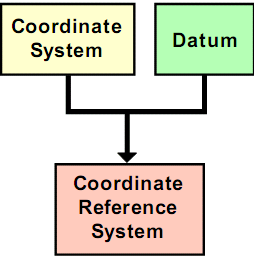
\includegraphics[width=0.3\textwidth]{Figures/coordinate system-datum_nikolli2011.png}
	\caption{A coordinate reference system combines a coordinate system with a datum, which gives the relationship of the coordinate system to the surface and shape of the Earth. Retrieved from \cite{nikolli_CRS_2011}.
		\label{fig:crs-datum}}
\end{figure}

A projection is the change of the representation of locations from one coordinate system to another. Sometimes it is more convenient to work with a flattened 2D projection of a datum rather than its spherical coordinates. With this, we project the coordinates into Cartesian $x$ and $y$ meters. We take $x=$ Easting and $y=$ Northing, in the order $(x, y)$, in meters from some origin. When we do a projection, we must make some compromise because it is not possible to make a perfect flat version of an ellipsoid surface. All projections of locations on the Earth into a two-dimensional plane are distortions as something always will be distorted \cite{lapaine_choosing_2017}. A good projection to use is one of the Universal Transverse Mercator (UTM) family. UTM splits the Earth's surface into state-sized regions, and defines separate projection for each one, to minimize the distortion there (see Figure \ref{fig:utm-zones}).

\begin{figure}[h!]
	\centering
	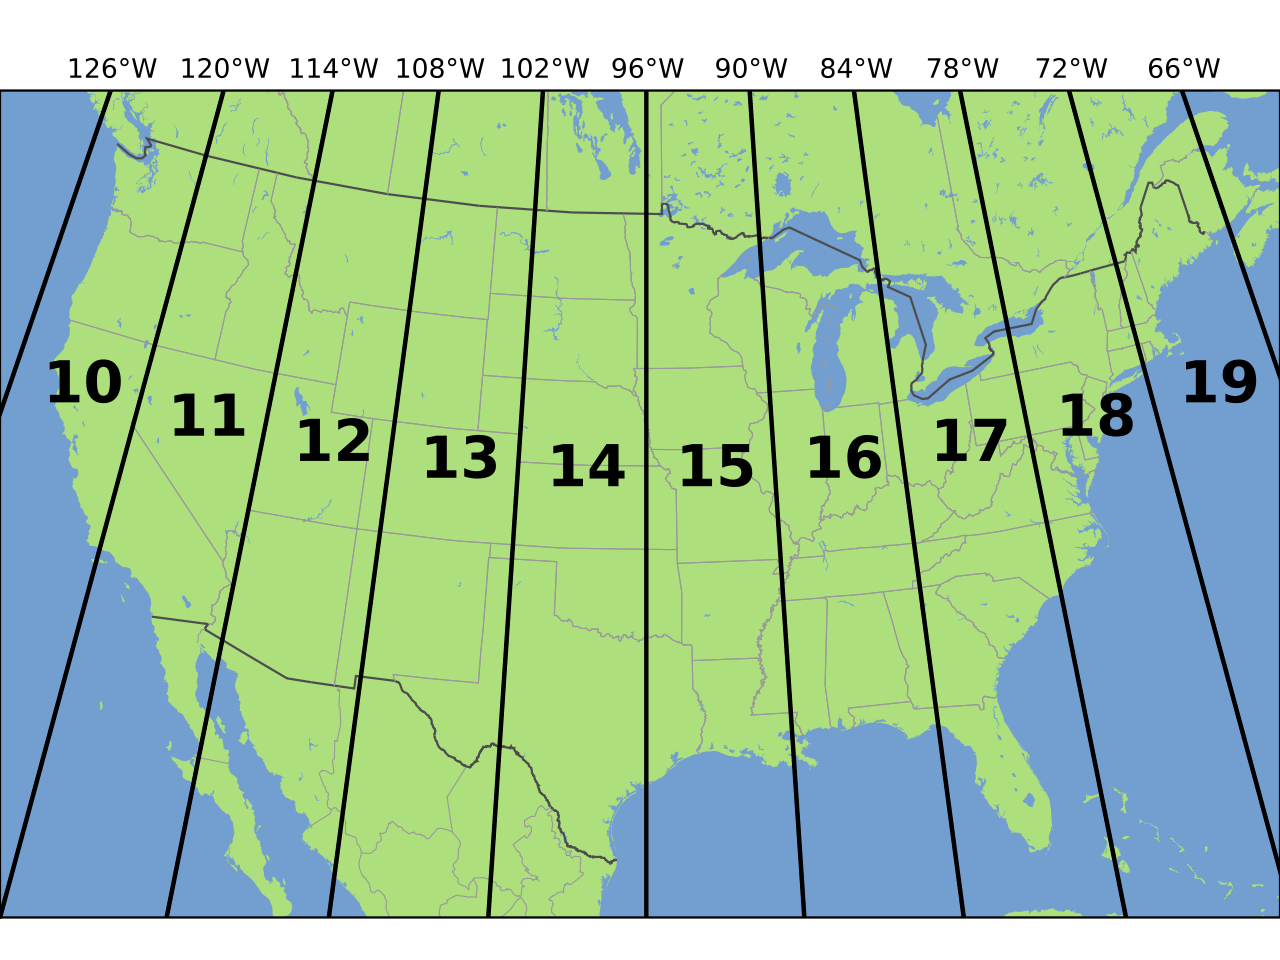
\includegraphics[width=0.3\textwidth]{Figures/UTM-zones.png}
	\caption{UTM zones across the continental United States. Source: \cite{chrismurf_2009}.
		\label{fig:utm-zones}}
\end{figure}

With geographic data it is common to work in only two of the three dimensions. Two dimensional space support three basic types of spatial entity \cite{iso_simple_features}:

\begin{itemize}
	\item points - having a location
	\item lines - comprising two or more locations in an ordered sequence
	\item polygons - areas defined by three or more vertex locations in an ordered sequence
\end{itemize}

\section{Geographic Information Systems (GIS)}

A Geographic Information System (GIS) is any system that is specifically designed to work with spatial data. GIS systems are implementations of some standard tasks, which may be present in as programming language libraries or functions, and/or as graphical user interfaces \cite{fox_spatial_2018}. Standard tasks include:

\begin{itemize}
	\item converting datums and projections
	\item searching quickly for entities in particular regions
	\item searching quickly for entities with spatial relationships to other entities
	\item handling lots of data at large and small scales
	\item geographical data visualizations
	\item converting between standard spatial data file formats
\end{itemize}

\section{Spatial files}

Shapefiles are a storage format for the Open Geo-spatial Consortium (OGC) definition: points, lines, and polygons. They are small collections of related files, usually stored together in a directory. The main file has a \textit{.shp} extension and stores the actual feature geometries. Other files that may appear along with it include \textit{.dbf} (associated non-spatial properties data), \textit{.shx} (indexing structure), and \textit{.prj} (datum/projection information) \cite{fox_spatial_2018}.

GeoJSON and Well-Known Text (WKT) are alternatives for storing such data. Most GIS systems can convert between those formats.

\section{OpenStreetMap}

OpenStreetMap (OSM) is a collaborative worldwide mapping project that provides a free and publicly editable map of the world. In February 2021, there were over 7M registered contributors, as outlined on the OSM wiki \cite{osm-wiki}.

In Mexico, OSM imported the 2015 INEGI's Marco Geoestadístico Nacional (MGN) and the Red Nacional de Caminos (RNC) road data during the years 2015 and 2016 as part of the two OSM projects: Mexico Main Road Network Import Project \cite{osm_RNC_project}, and Mexico's Administrative Divisions Import Project \cite{osm_MGN_project}. Additionally, individual contributions have been made from OSM members to keep updated and accurate the data.
Acquiring the spatial data from OSM is made via an API, called Overpass, to retrieve any data in the database. However, its usage and syntax are somewhat difficult and there are other services available that can simplify the process.

\section{Network Analysis Tools}


\subsection{NetworkX}

NetworkX is a free, open-source Python language package for the creation, manipulation, and study of the structure, dynamics, and functions of complex networks \cite{hagberg-schult-swart-networkx_2008, networkx_doc}. It provides data structures for graphs, digraphs, and multigraph, and implementations of many of the algorithms used in network science. These algorithms are implemented for structure and analysis measures, such as shortest paths, betweenness centrality, clustering, degree distribution and many more.

In addition NetworkX can read and write various graphs formats (e.g., adjacency list, edge list, GEXF, GML, pickle, GraphML, JSON, LEDA, YAML, SparseGraph6, Pajek, and GIS Shapefile), and provides generators for classic graphs, random graphs, and synthetic networks.


\subsection{GeoPandas}

GeoPandas 

\subsection{OSMnx}

\subsection{Gephi}

\subsection{NetworKit}

\subsection{PySAL}

